\documentclass[a4paper, 12pt]{report}

\usepackage[francais]{babel} % caractéres spéciaux en franéais

\usepackage[utf8]{inputenc}
\usepackage[T1]{fontenc} % police compatible français
\usepackage{lmodern}
\usepackage{amsmath}
\usepackage{amsfonts}
\usepackage{breqn}
\usepackage[parfill]{parskip}


\usepackage{graphicx}
\usepackage{float}
\usepackage{tikz}

\newcommand{\code}[1]{\textsf{#1}}

\renewcommand{\thepart}{\arabic{part}}
\renewcommand{\thesection}{\arabic{section}}
\renewcommand{\thesection}{\thepart.\arabic{section}}

\tikzset{every label/.style={font=\footnotesize,inner sep=1pt}}
\newcommand{\stencilpt}[4][]{\node[circle,fill,draw,inner sep=1.5pt,label={#4},#1] at (#2) (#3) {}}


\begin{document}

\begin{titlepage}

\newcommand{\HRule}{\rule{\linewidth}{0.5mm}} % Defines a new command for the horizontal lines, change thickness here

\center % Center everything on the page

%----------------------------------------------------------------------------------------
%   HEADING SECTIONS
%----------------------------------------------------------------------------------------

\textsc{\LARGE Université catholique de Louvain}\\[0.5cm] % Name of your university/college
\textsc{\Large Ecole de physique}\\[1.5cm] % Major heading such as course name
\textsc{\Large Simulation numérique en physique [\textsc{\normalsize LPHY2371}]}\\[0.5cm]
 % Minor heading such as course title

%----------------------------------------------------------------------------------------
%   TITLE SECTION
%----------------------------------------------------------------------------------------

\HRule \\[0.4cm]
{ \huge \bfseries Equation d'Advection-Diffusion et Prédictibilité}\\[0.4cm] % Title of your document
\HRule \\[1.5cm]

%----------------------------------------------------------------------------------------
%   AUTHOR SECTION
%----------------------------------------------------------------------------------------

\begin{minipage}[t]{0.6\textwidth}
\begin{flushleft} \large
\begin{tabbing}
\emph{Auteurs:}\\
Arnaud \hspace{0.1cm}\= \textsc{Schils}\\ % Your name
Valéry \> \textsc{Materne}
\end{tabbing}
\end{flushleft}
\end{minipage}
~
\begin{minipage}[t]{0.6\textwidth}
\begin{flushright} \large
\emph{Enseignant:} \\
Pr. Michel \textsc{Crucifix} % Supervisor's Name
\end{flushright}
\end{minipage}\\[1.5cm]

% If you don't want a supervisor, uncomment the two lines below and remove the section above
%\Large \emph{Author:}\\
%John \textsc{Smith}\\[3cm] % Your name

%----------------------------------------------------------------------------------------
%   DATE SECTION
%----------------------------------------------------------------------------------------

{\large Décembre 2016}\\[1.5cm] % Date, change the \today to a set date if you want to be precise

%----------------------------------------------------------------------------------------
%   LOGO SECTION
%----------------------------------------------------------------------------------------


\includegraphics[width=4cm]{Logo_UCL_SCIENCES.jpg}\\[1cm] % Include a department/university logo - this will require the graphicx package

%----------------------------------------------------------------------------------------

\vfill % Fill the rest of the page with whitespace

\end{titlepage}

\part{Equation d'Advection-Diffusion}

%\section*{Introduction}


\section{Fournissez un schéma numérique explicite d'ordre $\mathcal{O}(h+k)$.
Donnez-en le stencil. Nous pouvons introduire les facteurs $\lambda_d = Dk/h^2$,
$\lambda_a = ak/h$ et $\lambda_b = bk$. Quelles importances ces facteurs
 ont-ils pour la condition de stabilité?}

Dans cette section un schéma numérique explicite est fourni pour l'équation
aux dérivées partielles suivantes:

\begin{equation}
D \frac{\partial^2 u(x,t)}{\partial x^2} - a \frac{\partial u(x,t)}{\partial x} - b u(x,t) = \frac{\partial u(x,t)}{\partial t}
\label{eq:adv_diff}
\end{equation}

où $D, a$, $b$ sont des constantes et $D$ est positive. Dans la suite de ce texte les dépendances en $x$ et $t$
de la fonction $u$ ne seront pas toujours mentionnées explicitement.

\subsection*{Schéma numérique explicite}

Les dérivées de l'équation \eqref{eq:adv_diff} sont remplacées par leurs expressions
en différences finies. Soient $u(x_{\textsl{i}}, t_{\textsl{j}}) \equiv U_{\textsl{i},\textsl{j}}$, $h$ le pas d'espace
et $k$ le pas de temps, ces expressions sont:

\begin{align}
  \frac{\partial^2 u (x,t)}{\partial x^2} \biggr |_{x=x_{\textsl{i}}, t=t_{\textsl{j}}} &=& \frac{U_{\textsl{i}+1,\textsl{j}} - 2 U_{\textsl{i},\textsl{j}} + U_{\textsl{i}-1,\textsl{j}}}{h^2} + \mathcal{O}(h^2)\\
  \frac{\partial u (x,t)}{\partial x} \biggr |_{x=x_{\textsl{i}}, t=t_{\textsl{j}}} &=& \frac{U_{\textsl{i}+1,\textsl{j}} - U_{\textsl{i},\textsl{j}}}{h} + \mathcal{O}(h)\\
  \frac{\partial u (x,t)}{\partial t} \biggr |_{x=x_{\textsl{i}}, t=t_{\textsl{j}}} &=& \frac{U_{\textsl{i},\textsl{j}+1} - U_{\textsl{i},\textsl{j}}}{k} + \mathcal{O}(k) \;.
\end{align}

Nous avons pris une différence centrée pour la dérivée seconde par rapport à $x$ et une différence avant pour les dérivées premières par rapport à $x$ et $t$. Notons que pour la dérivée seconde par rapport à $x$, la formule à trois points d'ordre $\mathcal{O}(h^2)$ a été choisie au lieu de celles d'ordre $\mathcal{O}(h)$ afin d'obtenir à la fin une matrice tridiagonale. En injectant ces différences finies dans l'équation \eqref{eq:adv_diff} on obtient:

\begin{multline}
D \frac{U_{\textsl{i}+1,\textsl{j}} - 2 U_{\textsl{i},\textsl{j}} + U_{\textsl{i}-1,\textsl{j}}}{h^2} + \mathcal{O}(h^2) - a \frac{U_{\textsl{i}+1,\textsl{j}} - U_{\textsl{i},\textsl{j}}}{h} + \mathcal{O}(h) - b U_{\textsl{i},\textsl{j}}\\
= \frac{U_{\textsl{i},\textsl{j}+1} - U_{\textsl{i},\textsl{j}}}{k} + \mathcal{O}(k) \;.
\end{multline}

En multipliant l'expression par le pas de temps $k$, en isolant $U_{\textsl{i},\textsl{j}+1}$ et
en négligeant l'erreur en $\mathcal{O}(h^2)$ car elle est d'ordre supérieur à $\mathcal{O}(h)$
on obtient:

\begin{multline}
  U_{\textsl{i},\textsl{j}+1} = \frac{Dk}{h^2} (U_{\textsl{i}+1,\textsl{j}} - 2 U_{\textsl{i},\textsl{j}} + U_{\textsl{i}-1,\textsl{j}}) - \frac{ak}{h} (U_{\textsl{i}+1,\textsl{j}} - U_{\textsl{i},\textsl{j}}) - bk U_{\textsl{i},\textsl{j}} + U_{\textsl{i},\textsl{j}}\\
  + \mathcal{O}(h+k) \;.
\end{multline}

En définissant $\lambda_d = \frac{Dk}{h^2}$, $\lambda_a = \frac{ak}{h}$ et
$\lambda_b = bk$ l'expression devient:

\begin{multline}
  U_{\textsl{i},\textsl{j}+1} = \lambda_d (U_{\textsl{i}+1,\textsl{j}} - 2 U_{\textsl{i},\textsl{j}} + U_{\textsl{i}-1,\textsl{j}}) - \lambda_a (U_{\textsl{i}+1,\textsl{j}} - U_{\textsl{i},\textsl{j}}) - \lambda_b U_{\textsl{i},\textsl{j}} + U_{\textsl{i},\textsl{j}}\\
  + \mathcal{O}(h+k) \;.
\end{multline}

Sans spécifier l'ordre de l'erreur et en réarrangeant l'expression on a:

\begin{equation}
  U_{\textsl{i},\textsl{j}+1} = U_{\textsl{i}-1,\textsl{j}} \lambda_d + U_{\textsl{i},\textsl{j}} (-2 \lambda_d + \lambda_a - \lambda_b +1) + U_{\textsl{i}+1, \textsl{j}} (\lambda_d - \lambda_a)\;.
  \label{eq:schema_num_sans_erreur}
\end{equation}

En imposant les conditions aux bords constantes $\forall \textsl{j}, U_{0,\textsl{j}} = 0$
et $\forall \textsl{j}, U_{N+1,\textsl{j}} = 0$, le schéma numérique peut s'écrire
sous forme matricielle comme ceci:

\begin{equation}
  M =
  \begin{pmatrix}
     1 & 0 & ... & 0 & 0 \\
     \lambda_d & \ -2 \lambda_d + \lambda_a - \lambda_b + 1 \ & \lambda_d-\lambda_a &  0 & ...\\
     . & . & . &  . & .\\
     . & . & . &  . & .\\
     . & . & . &  . & .\\
     0 & ... & \lambda_d & \ -2 \lambda_d + \lambda_a - \lambda_b + 1 \ & \lambda_d-\lambda_a\\
     0 & 0 & ... & 0 & 1
  \end{pmatrix}
\end{equation}

\begin{equation}
\begin{pmatrix}
   U_{0,\textsl{j}+1} \\
   U_{1,\textsl{j}+1} \\
   .\\
   .\\
   .\\
   U_{N,\textsl{j}+1}\\
   U_{N+1,\textsl{j}+1}
\end{pmatrix}
=
M
\begin{pmatrix}
   U_{0,\textsl{j}} \\
   U_{1,\textsl{j}} \\
   .\\
   .\\
   .\\
   U_{N,\textsl{j}}\\
   U_{N+1,\textsl{j}}
\end{pmatrix}
\end{equation}

où $M$ est une matrice tridiagonale. Notons que les $U_{\textsl{i},0}$ sont connus
grâce aux conditions initiales.

\subsection*{Stencil}

Le stencil de ce schéma explicite est présenté
à la figure \ref{fig:stencil_schema_explicite}. Chaque $U_{\textsl{i},\textsl{j}+1}$ dépend
en effet des $U_{\textsl{i}-1,\textsl{j}}$, $U_{\textsl{i},\textsl{j}}$ et $U_{\textsl{i}+1,\textsl{j}}$.

\begin{figure}[H]
  \center
\begin{tikzpicture}

  \stencilpt{0, 2}{ij+1}{$x_{\textsl{i}},t_{\textsl{j}+1}$};
  \stencilpt{0, 1}{ij}{$x_{\textsl{i}},t_{\textsl{j}}$};
  \stencilpt{-2, 1}{i-1j}{$x_{\textsl{i}-1},t_{\textsl{j}}$};
  \stencilpt{2, 1}{i+1j}{$x_{\textsl{i}+1},t_{\textsl{j}}$};
  \stencilpt{0,0}{ij-1}{$x_{\textsl{i}},t_{\textsl{j}-1}$};
  \stencilpt{2,0}{i+1j-1}{$x_{\textsl{i}+1},t_{\textsl{j}-1}$};
  \stencilpt{-2,0}{i-1j-1}{$x_{\textsl{i}-1},t_{\textsl{j}-1}$};
  \stencilpt{4,0}{i+2j-1}{$x_{\textsl{i}+2},t_{\textsl{j}-1}$};
  \stencilpt{-4,0}{i-2j-1}{$x_{\textsl{i}-2},t_{\textsl{j}-1}$};
  \stencilpt{-6,-1}{l}{$x_{\textsl{i}}-(\textsl{j}+1)h, t_0$};
  \stencilpt{-4,-1}{l2}{};
  \stencilpt{-2,-1}{l3}{};
  \stencilpt{0,-1}{l4}{$x_{\textsl{i}}, t_0$};
  \stencilpt{2,-1}{l5}{};
  \stencilpt{4,-1}{l6}{};
  \stencilpt{6,-1}{l7}{$x_{\textsl{i}}+(\textsl{j}+1)h, t_0$};

  \draw (ij+1)   -- (ij)
        (ij) -- (i-1j)
        (i-1j)   -- (i+1j)
        (i-1j-1) -- (i-1j)
        (ij-1) -- (ij)
        (i+1j-1) -- (i+1j)
        (i-2j-1) -- (i-1j-1)
        (i-1j-1) -- (ij-1)
        (ij-1) -- (i+1j-1)
        (i+1j-1) -- (i+2j-1)
        (l) -- (l2)
        (l2) -- (l3)
        (l3) -- (l4)
        (l4) -- (l5)
        (l5) -- (l6)
        (l6) -- (l7)
        (l2) -- (i-2j-1)
        (l3) -- (i-1j-1)
        (l4) -- (ij-1)
        (l5) -- (i+1j-1)
        (l6) -- (i+2j-1);
\end{tikzpicture}
\caption{Stencil du schéma numérique explicite.}
\label{fig:stencil_schema_explicite}
\end{figure}

\subsection*{Importance des facteurs $\lambda_d, \lambda_a$ et $\lambda_b$ pour
la condition de stabilité}

Ces facteurs sont reliés aux conditions de stabilité
de la méthode aux différences finies. Pour le montrer, introduisons dans notre
schéma numérique une solution de la forme:

\begin{equation}
U_{\textsl{i},\textsl{j}} = w_{\textsl{j}} \exp (i r x_{\textsl{i}}) \;,
\label{eq:stabilite_expl_sol}
\end{equation}

où $i \equiv \sqrt{-1}$. Nous injectons cette solution dans l'équation \eqref{eq:schema_num_sans_erreur}, on obtient :

\begin{multline}
  w_{\textsl{j+1}} e^{irx_{\textsl{i}}} = w_{\textsl{j}} e^{irx_{\textsl{i-1}}}
  \lambda_d + w_{\textsl{j}} e^{irx_{\textsl{i}}} (-2 \lambda_d + \lambda_a - \lambda_b +1)\\
  + w_{\textsl{j}} e^{irx_{\textsl{i+1}}} (\lambda_d - \lambda_a)
\end{multline}

En tenant compte du pas d'espace $x_{\textsl{i+1}}- x_{\textsl{i}}= h$, après calcul :

\begin{multline}
  w_{\textsl{j+1}} = w_{\textsl{j}} e^{-irh} \lambda_d
  + w_{\textsl{j}} (-2 \lambda_d + \lambda_a - \lambda_b +1)
  + w_{\textsl{j}} e^{irh} (\lambda_d - \lambda_a)\\
  = w_{\textsl{j}} \left ( \lambda_d \left ( e^{-irh} -2 + e^{irh} \right )
  + \lambda_a \left (1- e^{irh} \right ) - \lambda_b + 1\right )\\
  = w_{\textsl{j}} \left ( 1 + \lambda_d \left (2\cos(rh) -2  \right )
  + \lambda_a \left (1- e^{irh} \right ) - \lambda_b \right )\\
  = w_{\textsl{j}} \left ( 1 - 4 \lambda_d \sin^2(rh/2)
  + \lambda_a \left (1- e^{irh} \right ) - \lambda_b \right )\;.
\end{multline}

Il s'agit d'une equation au différences, que l'on peut résoudre en posant :

\begin{equation}
  w_{\textsl{j}} = w_{0}\kappa^{\textsl{j}} \;.
\end{equation}

On obtient alors $\kappa \equiv  1 - 4 \lambda_d \sin^2(rh/2) + \lambda_a \left (1- e^{irh} \right ) - \lambda_b$ qui est complexe. La condition de stabilité se ramène alors à:

\begin{equation}
|\kappa|^2 = \left ( 1 - 4 \lambda_d \sin^2(rh/2) + \lambda_a \left (1- \cos(rh) \right ) - \lambda_b \right )^2+ \lambda_a^2 \sin^2(rh) \le 1\;.
\end{equation}

Les valeurs des paramètres $\lambda_d, \lambda_a$ et $\lambda_b$ déterminent donc
la stabilité du schéma numérique. L'expression peut se réécrire:

\begin{equation}
\boxed{|\kappa|^2 = \left ( 1 + 2 \sin^2(rh/2) \left (\lambda_a-2\lambda_d \right )- \lambda_b \right )^2+ \lambda_a^2 \sin^2(rh) \le 1}\;.
\label{eq:kappa_squared}
\end{equation}

L'expression est trop compliquée pour pouvoir trouver une condition exacte
de stabilité sur les différents $\lambda$. Par contre, on peut trouver
des conditions qui guarantissent stabilité pour certaines valeurs des $\lambda$
sans pour autant pouvoir déterminer toutes les combinaisons de $\lambda$ stables.

Une condition pessimiste peut êre obtenue en posant les valeurs des sinus à celles
qui maximisent chacun des termes de l'équation \eqref{eq:kappa_squared}.
Le pire cas pour le terme de droite est toujours $\sin^2(rh)=1$. Pour le terme
de gauche, cela dépend des signes et valeurs respectives des différents
$\lambda$. Deux cas peuvent être distingués.

Si $|1-\lambda_b| > |1-\lambda_b + 2 (\lambda_a-2\lambda_d)|$, le terme de gauche
est maximisé si $\sin^2(rh/2)=0$. La condition pessimiste de stabilité
est alors:

\begin{equation}
  \left (1-\lambda_b \right )^2 + \lambda_a^2 \le 1 \implies \lambda_b (\lambda_b-2) + \lambda_a^2 \le 0
\end{equation}

Sinon, le terme de gauche est maximisé si $\sin^2(rh/2)=1$. La condition
pessimiste de stabilité est alors dans ce deuxième cas:

\begin{equation}
    \left ( 1+2(\lambda_a-2\lambda_d) - \lambda_b \right )^2 + \lambda_a^2 \le 1 \;.
    \label{eq:expl_stabilite_cond_2}
\end{equation}

A partir de ces conditions, une fonction Matlab \code{is\_stable\_expl} a été
implémentée. Lorsque celle-ci renvoie $1$ (le booléen \code{true}) cela signifie
que la méthode est stable. Si elle renvoie $0$ (le booléen \code{false}), cela
ne signifie rien (on ne sait pas si la méthode sera stable ou non).

Il a été vérifié pour toutes les combinaisons de paramètres possibles parmi $a \in \{-10, 1, 10\}$,
$b \in \{-10, 1, 10\}, D \in \{1, 10, 50\}, h \in \{0.0001, 0.001, 0.01\}$
et $k \in \{0.000001, 0.00001, 0.0001\}$ que la méthode numérique est
effectivement stable lorsque la fonction \code{is\_stable\_expl} renvoie \code{true}.


\section{Fournissez la solution analytique de l'équation, ainsi que la relation
de dispersion. Discutez brièvement les cas particuliers déjà vus au cours (D=0, b=0, etc.).}

L'équation aux dérivées partielles à résoudre est l'équation \eqref{eq:adv_diff}. Les conditions
aux bords suivantes sont imposées:

\begin{equation}
  \left \{
  \begin{aligned}
    u(x,0) = g(x)\\
    u(0,t) = u(l,t) = 0
  \end{aligned}
  \right.
\end{equation}

où $l > 0$. La solution $u$ est donc recherchée dans le domaine:

\begin{equation}
  \left \{
  \begin{aligned}
    t \ge 0\\
    0 < x < l
  \end{aligned}
  \right.
\end{equation}

L'équation \eqref{eq:adv_diff} peut-être résolue par la méthode de séparation de
variables. La solution $u$ est supposée être de la forme:

\begin{equation}
  u(x,t) = v(x) w(t)
\end{equation}

En injectant cette forme de $u$ dans l'équation \eqref{eq:adv_diff} on obtient:

\begin{equation}
D w(t) \frac{\partial^2 v(x)}{\partial x^2} - a w(t) \frac{\partial v(x)}{\partial x} - b v(x) w(t) = v(x) \frac{\partial w(t)}{\partial t}
\end{equation}

En divisant cette équation par $v(x) w(t)$ on obtient:

\begin{equation}
  \frac{D}{v} \frac{\partial^2 v}{\partial x^2} - \frac{a}{v} \frac{\partial v}{\partial x} -b = \frac{1}{w} \frac{\partial w}{\partial t} \equiv C_1
\end{equation}

Chaque partie de l'équation est en effet égale à une constante $C_1$ puisque
la partie gauche ne dépend que de $x$ et la partie droite ne dépend que de $t$.
L'équation peut maintenant être résolue en résolvant séparément la partie
qui dépend du temps $t$ et la partie qui dépend de la position $x$. Pour la
partie dépendante du temps on a:

\begin{align}
\frac{1}{w} \frac{\partial w}{\partial t} = C_1\\
\frac{\partial w}{\partial t} = C_1 w\\
w(t) = C_{2} e^{C_1 t}
\end{align}

où $C_{2}$ est une constante. Pour la partie dépendante de la position $x$
on a:

\begin{align}
  \frac{D}{v} \frac{\partial^2v}{\partial x^2} - \frac{a}{v} \frac{\partial v}{\partial x} = C_1 + b\\
  D \frac{d^2v}{d x^2} - a \frac{d v}{d x} - (C_1 + b) v = 0
\end{align}

C'est une équation différentielle linéaire homogène du 2ème ordre. Sa solution
dépend donc de son polynôme caractéristique:

\begin{align}
  D r^2 - a r - (C_1 + b) = 0\\
  \rho = a^2 + 4 D (C_1 + b)
\end{align}

Les deux racines de ce polynôme sont:

\begin{equation}
   r_{1,2} = \frac{a \pm \sqrt{\rho}}{2 D}
 \end{equation}

En fonction du signe de $\rho$ la solution de l'équation peut avoir trois formes.

\underline{Si $\rho > 0$}

\begin{equation}
  v(x) = C_3 e^{r_1 x} + C_4 e^{r_2 x}
\end{equation}

où $C_3$ et $C_4$ sont des constantes. En utilisant la condition au bord
$u(0,t) = 0 = v(0) w(t) \implies v(0) = 0$ on a:

\begin{equation}
  C_4 = -C_3 \implies  v(x) = C_3 (e^{r_1 x} - e^{r_2 x})
\end{equation}

Et en utilisant la condition au bord $u(l,t) = 0 = v(l) w(t) \implies v(l) = 0$ on a:

\begin{equation}
  C_3 (e^{r_1 l} - e^{r_2 l}) = 0 \implies C_{3} = 0 \implies v(x) = 0
\end{equation}

Cette solution n'est donc pas intéressante par rapport à nos conditions aux bords.

\underline{Si $\rho = 0, r_1 = r_2 \equiv r$}

\begin{equation}
  v(x) = (C_3 + C_4 x) e^{r x}
\end{equation}

où $C_3$ et $C_4$ sont des constantes. En utilisant la condition au bord
$u(0,t) = 0 = v(0) w(t) \implies v(0) = 0$ on a:

\begin{equation}
  C_3 = 0 \implies   v(x) = C_4 x e^{r x}
\end{equation}

Et en utilisant la condition au bord $u(l,t) = 0 = v(l) w(t) \implies v(l) = 0$ on a:

\begin{equation}
  C_4 l e^{r l} = 0 \implies C_4 = 0 \implies v(x) = 0
\end{equation}

Cette solution n'est donc pas intéressante par rapport à nos conditions aux bords.

\underline{Si $\rho < 0$}

On définit
\begin{equation}
r_{1,2} \equiv \alpha \pm i \beta
\end{equation}

avec

\begin{eqnarray}
  \alpha & = & \frac{a}{2 D}\;,\\
  \beta & = & \frac{\sqrt{-a^{2} - 4 D (C_{1} + b)}}{2 D}\;.\label{beta}
\end{eqnarray}

On a alors comme solution pour $v(x)$ :

\begin{equation}
  v(x) = (C_3 \cos(\beta x) + C_4 \sin(\beta x)) e^{\alpha x}\;.
\end{equation}

En utilisant la condition au bord $u(0,t) = 0 = v(0) w(t) \implies v(0) = 0$ on a:

\begin{equation}
  C_3 = 0 \implies v(x) = C_4 \sin(\beta x) e^{\alpha x}
\end{equation}

Et en utilisant la condition au bord $u(l,t) = 0 = v(l) w(t) \implies v(l) = 0$ on a:

\begin{equation}
  \sin(\beta l) = 0 \implies \beta l = m \pi \implies \beta = \frac{m \pi}{l}, m \in \mathbb{N}^{\ast}\;.
\end{equation}

On notera que $\beta > 0$ car $\rho < 0$ et $D > 0$. \\
La solution générale pour la partie de l'équation dépendante de la position est
donc:

\begin{equation}
  v(x) = \sum_{m=1}^{\infty} C_{4_m} \sin \left (\frac{m \pi x}{l} \right ) e^{\alpha x}
\end{equation}

où les $C_{4_m}$ sont des constantes. Utilisons maintenant la condition au bord
$u(x,0) = g(x)$ afin de déterminer les valeurs de ces constantes $C_{4_m}$:

\begin{equation}
  u(x,0) = v(x) w(0) = v(x) C_{2} = g(x)\;.
\end{equation}

On a alors,

\begin{equation}
  g(x) = \sum_{m=1}^{\infty} C_{4_m}C_{2} \sin \left (\frac{m \pi x}{l} \right ) e^{\alpha x}\;.
\end{equation}

En définissant $C_m = C_{4_m}C_{2}$ on obtient:

\begin{equation}
  g(x) = \sum_{m=1}^{\infty} C_m \sin \left (\frac{m \pi x}{l} \right ) e^{\alpha x}
\end{equation}

On voit dès lors que les coefficients $C_m$ sont obtenus
en projetant la fonction $g(x)e^{-\alpha x}$ sur la base des fonctions $\sin \left (\frac{m \pi x}{l} \right )$:

\begin{equation}
  C_m = \frac{2}{l} \int_0^l g(x) \sin \left (\frac{m \pi x}{l} \right ) e^{-\alpha x} dx
\end{equation}

%Puisque le terme de la somme pour $m=0$ est égal à zéro, et que la fonction
%sinus est impaire:

%\begin{align}
%  \tilde{C}_{4_{(-m)}} = \frac{2}{l} \int_0^l g(x) \sin \left (\frac{-m \pi x}{l} \right ) e^{-\alpha x} dx = -\tilde{C}_{4_m}\\
%  \implies \tilde{C}_{4_{(-m)}} \sin \left (\frac{-m \pi x}{l} \right ) e^{\alpha x} = \tilde{C}_{4_m} \sin \left (\frac{m \pi x}{l} \right ) e^{\alpha x}
%\end{align}

%Et donc:

%\begin{equation}
%  g(x) = \sum_{m=1}^{\infty} 2 \tilde{C}_{4_m} \sin \left (\frac{m \pi x}{l} \right ) e^{\alpha x}
%\end{equation}

%En définissant $C^'_{4_m} = 2 \tilde{C}_{4_m}$ on peut écrire:

%\begin{equation}
%  g(x) = \sum_{m=1}^{\infty} C^'_{4_m} \sin \left (\frac{m \pi x}{l} \right ) e^{\alpha x}
%\end{equation}

%avec

%\begin{equation}
%  C^'_{4_m} =  \frac{2}{l} \int_0^l g(x) \sin \left (\frac{m \pi x}{l} \right ) e^{-\alpha x} dx
%\end{equation}

La fonction $u(x,t)$ peut alors s'écrire:

\begin{equation}
u(x,t) = \sum_{m=1}^{\infty} C_m \sin \left (\frac{m \pi x}{l} \right ) e^{\alpha x} e^{C_{1_m} t}
\end{equation}

Nous devons maintenant déterminer l'expression de la constante $C_{1_m}$ qui dépend de $\beta$ et donc de $m$. En partant de l'expression de $\beta$ \eqref{beta}, on obtient :

\begin{equation}
  C_{1_m}= \frac{-a^2 - 4D^{2}\beta^{2}}{4D}-b
\end{equation}
et avec $\beta = \frac{m \pi}{l}$, on a :
\begin{equation}
  C_{1_m}= - \frac{a^2}{4D} - \frac{D m^2 \pi^2}{l^2}-b\;.
\end{equation}

En injectant l'expression de $C_{1_m}$ dans celle de $u$ on a alors :

\begin{equation}
u(x,t) = \sum_{m=1}^{\infty} C_m \sin \left (\frac{m \pi x}{l} \right ) \exp \left ( \frac{a x}{2D} + \left ( - \frac{a^2}{4D} - \frac{D m^2 \pi^2}{l^2}-b \right ) t \right )
\end{equation}

\begin{equation}
  \boxed{u(x,t) = \sum_{m=1}^{\infty} C_m \sin \left (\frac{m \pi x}{l} \right ) \exp \left ( \frac{a}{2D} \left (x - \frac{a}{2} t \right ) - \left (\frac{D m^2 \pi^2}{l^2}+b \right ) t \right )\\
}
\label{eq:analy_sol}
\end{equation}

avec

\begin{equation}
  \boxed{C_m = \frac{2}{l} \int_0^l g(x) \sin \left (\frac{m \pi x}{l} \right ) \exp \left ( -\frac{a}{2D} x \right ) dx}\;.
\end{equation}


\subsection*{Relation de dispersion}

On utilise, comme solution à l'équation d'advection-diffusion \eqref{eq:adv_diff}, une onde plane de la forme :

\begin{equation}
  u(x,t) = e^{\dot{\imath}\left(kx-\omega t\right)}
\end{equation}

avec $k$ le nombre d'onde qui est relié à la longueur d'onde $\lambda$ par la relation $\lambda = 2\pi/k$ et $\omega$ la fréquence de l'onde.

On obtient alors l'expression suivante :

\begin{equation}
  \omega = ak-\dot{\imath}\left(Dk^{2}+b\right)
	\label{eq:dispersion}
\end{equation}

qui est la relation de dispersion de l'équation \eqref{eq:adv_diff}. Elle détermine la fréquence $\omega$ en fonction de $k$ pour une onde plane prise comme solution.

\subsection*{Cas particuliers}

Si $D=1$, $a=b=0$ on retrouve l'équation de la chaleur adimensionnelle et homogène:

\begin{equation}
  \frac{\partial^2 u(x,t)}{\partial x^2} = \frac{\partial u(x,t)}{\partial t}\;.
\end{equation}

En injectant ces valeurs de $D,a$ et $b$ dans l'équation \eqref{eq:analy_sol} on a:

 \begin{equation}
   u(x,t) = \sum_{m=1}^{\infty} C_m \sin \left (\frac{m \pi x}{l} \right ) \exp \left ( - \left (\frac{m^2 \pi^2}{l^2} \right ) t \right )
 \end{equation}

 avec

 \begin{equation}
   C_m = \frac{2}{l} \int_0^l g(x) \sin \left (\frac{m \pi x}{l} \right )  dx \;.
 \end{equation}

 On retombe donc bien sur la solution de l'équation de la chaleur adimensionnelle
 homogène du cours si l'on pose $l=1$.

Si $D=0=b$ on retrouve la forme générale de l'équation d'advection:

\begin{equation}
  \frac{\partial u(x,t)}{\partial t} + a \frac{\partial u(x,t)}{\partial x} = 0 \;.
  \label{eq:advection}
\end{equation}

La solution présentée à l'équation \eqref{eq:analy_sol} n'est alors plus valide
car celle-ci n'est valable que si $D>0$ et $\rho < 0$. La solution de
l'équation \eqref{eq:advection} est $u(x,t) = g(x-at)$ avec comme condition
initiale $u(x,0) = g(x)$ (démonstration faite en séance d'exercices).


\section{Fournissez un schéma implicite. Est-il toujours stable?}
\label{sec:implicite}

Le schéma implicite est obtenu en discrétisant l'Equation~\ref{eq:adv_diff}
de la façon suivante. La fonction $u$ est remplacée par l'image du point $(x_{\textsl{i}},t_{\textsl{j+1}})$
c'est à dire par $U_{\textsl{i},\textsl{j+1}}$. Les dérivées sont remplacées par leurs formulations discrètes
au temps $t_{j+1}$:

\begin{align}
  \frac{\partial^2 u (x,t)}{\partial x^2} \biggr |_{x=x_{\textsl{i}}, t=t_{\textsl{j+1}}} &=& \frac{U_{\textsl{i}+1,\textsl{j+1}} - 2 U_{\textsl{i},\textsl{j+1}} + U_{\textsl{i}-1,\textsl{j+1}}}{h^2} + \mathcal{O}(h^2)\\
  \frac{\partial u (x,t)}{\partial x} \biggr |_{x=x_{\textsl{i}}, t=t_{\textsl{j+1}}} &=& \frac{U_{\textsl{i}+1,\textsl{j+1}} - U_{\textsl{i},\textsl{j+1}}}{h} + \mathcal{O}(h)\\
  \frac{\partial u (x,t)}{\partial t} \biggr |_{x=x_{\textsl{i}}, t=t_{\textsl{j+1}}} &=& \frac{U_{\textsl{i},\textsl{j}+1} - U_{\textsl{i},\textsl{j}}}{k} + \mathcal{O}(k) \;.
\end{align}

On obtient alors:

\begin{multline}
\frac{U_{\textsl{i},\textsl{j+1}} - U_{\textsl{i},\textsl{j}}}{k} + \mathcal{O}(k)  = D \frac{U_{\textsl{i}+1,\textsl{j+1}} - 2 U_{\textsl{i},\textsl{j+1}} + U_{\textsl{i}-1,\textsl{j+1}}}{h^2}+ \mathcal{O}(h^2) \\
- a \frac{U_{\textsl{i+1},\textsl{j+1}} - U_{\textsl{i},\textsl{j+1}}}{h} + \mathcal{O}(h) - b U_{\textsl{i},\textsl{j+1}}\;.
\end{multline}

Le schéma est d'ordre $\mathcal{O}(h+k)$. En isolant $U_{\textsl{i},\textsl{j}}$
et en introduisant les quantités $\lambda_a$, $\lambda_b$ et $\lambda_d$ depuis
leurs définitions on obtient:

\begin{equation}
  U_{\textsl{i},\textsl{j}} = - \lambda_d U_{\textsl{i-1},\textsl{j+1}}
  +U_{\textsl{i},\textsl{j+1}} (1+ 2 \lambda_d + \lambda_b - \lambda_a)
  +U_{\textsl{i+1},\textsl{j+1}} (\lambda_a - \lambda_d)
  \label{eq:schema_implicite}
\end{equation}

La matrice $M$ correspondante est présentée ci-dessous.

\begin{equation}
  M =
  \begin{pmatrix}
     1 & 0 & ... & 0 & 0 \\
     -\lambda_d & \ 2 \lambda_d - \lambda_a + \lambda_b + 1 \ & \lambda_a-\lambda_d &  0 & ...\\
     . & . & . &  . & .\\
     . & . & . &  . & .\\
     . & . & . &  . & .\\
     0 & ... & -\lambda_d & \ 2 \lambda_d - \lambda_a + \lambda_b + 1 \ & \lambda_a-\lambda_d\\
     0 & 0 & ... & 0 & 1
  \end{pmatrix}
\end{equation}

\begin{equation}
\begin{pmatrix}
   U_{0,\textsl{j}+1} \\
   U_{1,\textsl{j}+1} \\
   .\\
   .\\
   .\\
   U_{N,\textsl{j}+1}\\
   U_{N+1,\textsl{j}+1}
\end{pmatrix}
=
M^{-1}
\begin{pmatrix}
   U_{0,\textsl{j}} \\
   U_{1,\textsl{j}} \\
   .\\
   .\\
   .\\
   U_{N,\textsl{j}}\\
   U_{N+1,\textsl{j}}
\end{pmatrix}
\end{equation}

où $M$ est une matrice tridiagonale. Notons que les $U_{\textsl{i},0}$ sont connus
grâce aux conditions initiales.

\subsection*{Stabilité}

Afin de trouver une condition de stabilité pour la méthode implicite injectons
l'équation \eqref{eq:stabilite_expl_sol} dans le schéma numérique implicite
(équation \eqref{eq:schema_implicite}). On obtient alors:

\begin{equation}
  w_{\textsl{j}} e^{irx_{\textsl{i}}} = -\lambda_d w_{\textsl{j+1}} e^{irx_{\textsl{i-1}}}
  + w_{\textsl{j+1}} e^{irx_{\textsl{i}}} (1+2 \lambda_d + \lambda_b - \lambda_a)
  +w_{\textsl{j+1}} e^{irx_{\textsl{i+1}}} (\lambda_a - \lambda_d) \;.
\end{equation}

\begin{equation}
  w_{\textsl{j}} = w_{\textsl{j+1}} \left (-\lambda_d e^{-irh} +1 + 2 \lambda_d+\lambda_b-\lambda_a + e^{irh} (\lambda_a - \lambda_d) \right )
\end{equation}

Et donc,

\begin{equation}
  w_{\textsl{j+1}} = \kappa w_{\textsl{j}} \Leftrightarrow w_{\textsl{j}} = \kappa w_{\textsl{j-1}} = \kappa^j w_0
\end{equation}

avec

\begin{equation}
\kappa \equiv \left [ -\lambda_d e^{-irh} +1 + 2 \lambda_d+\lambda_b-\lambda_a + e^{irh} (\lambda_a - \lambda_d) \right ]^{-1} \equiv \alpha^{-1}\;.
\end{equation}

On a,

\begin{multline}
  \alpha = -\lambda_d (2\cos(rh)-2) +1 +\lambda_b+\lambda_a ( e^{irh}-1)\\
  = 4 \lambda_d \sin^2(rh/2) +1 +\lambda_b -2 \lambda_a \sin^2(rh/2) +  i \lambda_a \sin(rh) \equiv a+ib\;.
\end{multline}

Afin que la méthode numérique soit stable on veut donc que

\begin{equation}
  |\kappa|^2 \le 1 \Leftrightarrow |\alpha^{-1}|^2 \le 1\;.
\end{equation}

Par ailleurs,

\begin{equation}
\alpha^{-1} = \frac{1}{a+ib} = \frac{a-ib}{a^2+b^2}\;.
\end{equation}

La condition de stabilité devient donc:

\begin{equation}
 \frac{1}{(a^2+b^2)^2}|a-ib|^2 = \frac{a^2+b^2}{(a^2+b^2)^2} = \frac{1}{a^2+b^2}  \le 1 \implies a^2+b^2 \ge 1\;.
\end{equation}

On a finalement:

\begin{equation}
\boxed{\left ( 2 \sin^2(rh/2) (2 \lambda_d - \lambda_a) +1 + \lambda_b \right )^2 + \lambda_a^2 \sin^2(rh) \ge 1}\;.
\end{equation}

Le schéma n'est donc pas toujours stable. En effet par exemple lorsque
$\sin^2(rh/2) = 0 = \sin^2(rh)$ et $\lambda_b = -1$. Ou encore lorsque
$\lambda_d = \lambda_a/2$, $\lambda_b = -1$ et $\lambda_a < 1$ (voir Figure~\ref{eq:impl_instable}).

\section{Illustrez votre propos avec plusieurs simulations numériques, comparant schémas numériques implicites et explicites.}

Pour tous les graphiques présentés dans cette section, la condition initiale
utilisée est $g(x) = 1+\cos(8x \pi /l+ \pi )$. On peut constater qu'elle satisfait
bien aux conditions aux bords imposées $g(0) = g(l) = 0$.

\begin{figure}[H]
  \center
  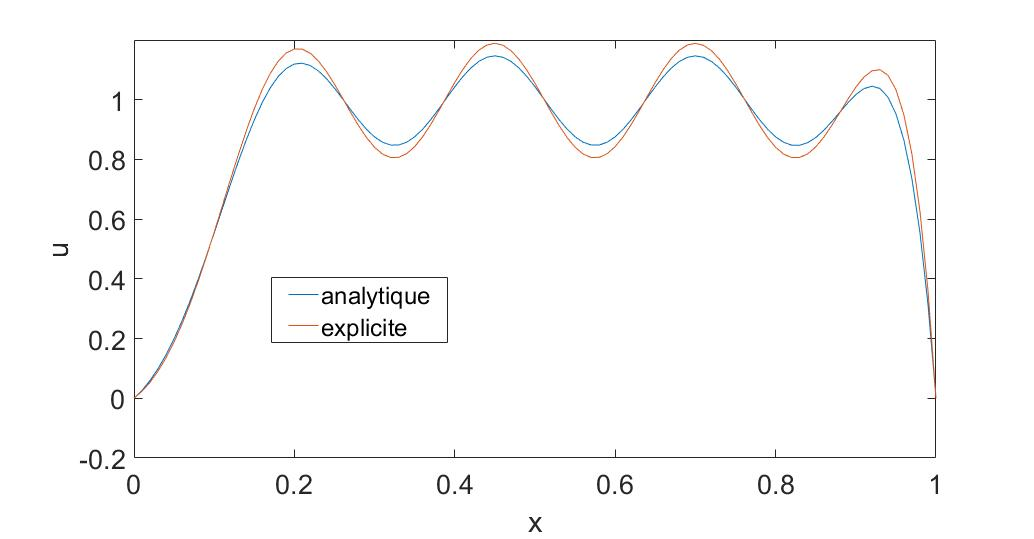
\includegraphics[scale=0.4]{images/analy_vs_expl_t_end_0dot003.jpg}
  \caption{Comparaison entre les solutions analytique et numérique explicite pour
  les paramètres $a=25$, $b=1$, $D=1$, $h=0.01$ et $k=0.00001$, au temps $t=0.003$.}
\end{figure}

\begin{figure}[H]
  \center
  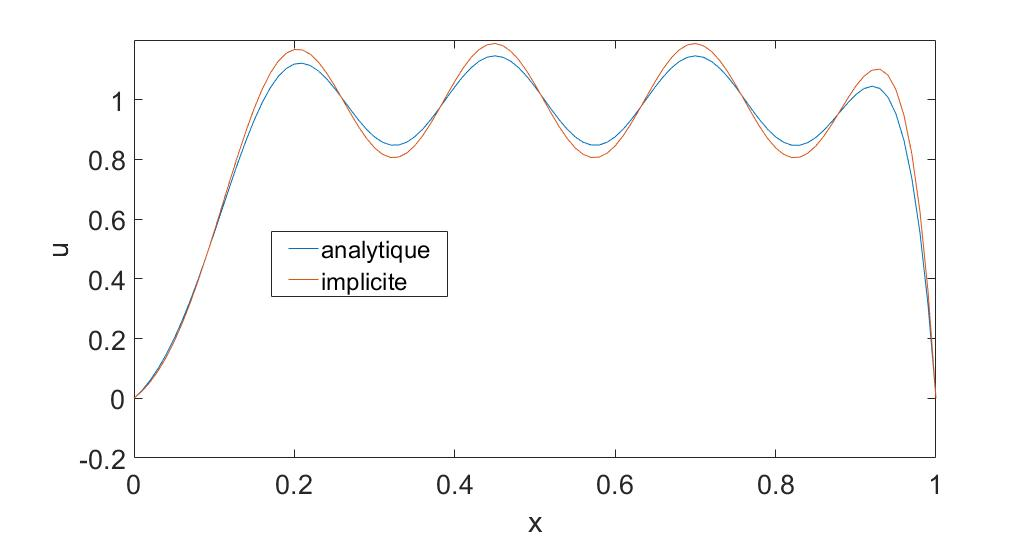
\includegraphics[scale=0.4]{images/analy_vs_impl_t_end_0dot003.jpg}
  \caption{Comparaison entre les solutions analytique et numérique implicite pour
  les paramètres $a=25$, $b=1$, $D=1$, $h=0.01$ et $k=0.00001$, au temps $t=0.003$.}
\end{figure}

\begin{figure}[H]
  \center
  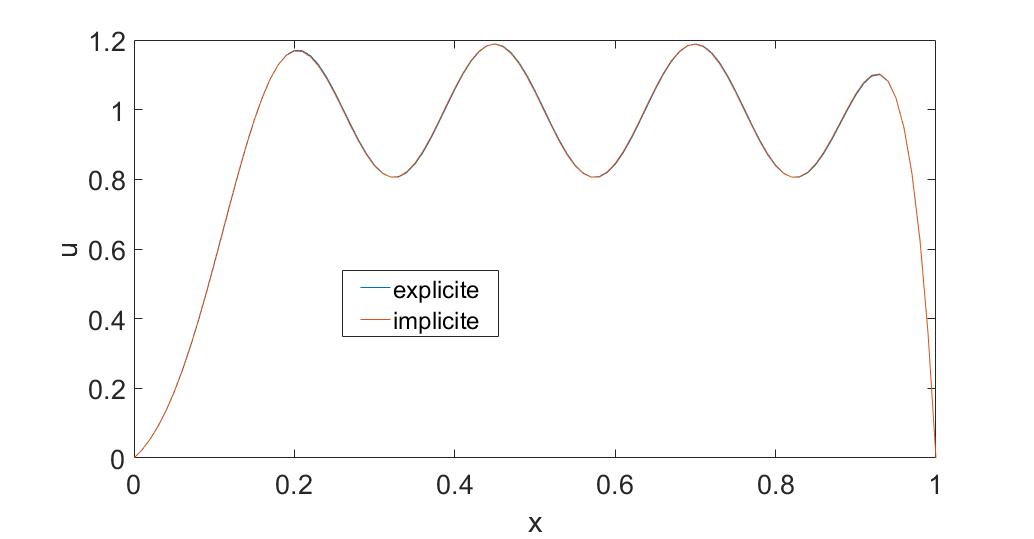
\includegraphics[scale=0.4]{images/expl_vs_impl_t_end_0dot003.jpg}
  \caption{Comparaison entre les solutions numériques implicite et explicite pour
  les paramètres $a=25$, $b=1$, $D=1$, $h=0.01$ et $k=0.00001$, au temps $t=0.003$.}
  \label{eq:expl_vs_impl_t0dot003}
\end{figure}

\begin{figure}[H]
  \center
  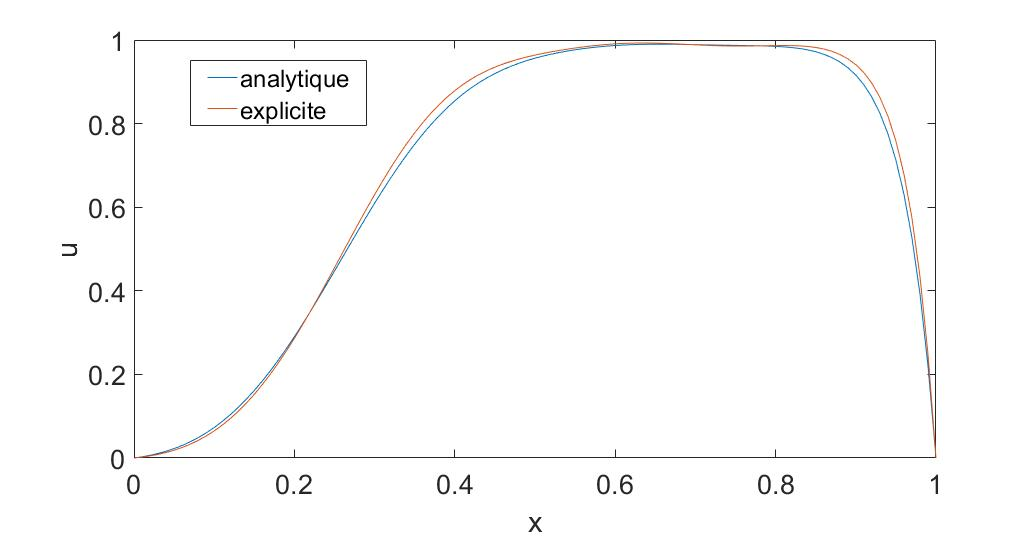
\includegraphics[scale=0.4]{images/analy_vs_expl_t_end_0dot01.jpg}
  \caption{Comparaison entre les solutions analytique et numérique explicite pour
  les paramètres $a=25$, $b=1$, $D=1$, $h=0.01$ et $k=0.00001$, au temps $t=0.01$.}
\end{figure}

\begin{figure}[H]
  \center
  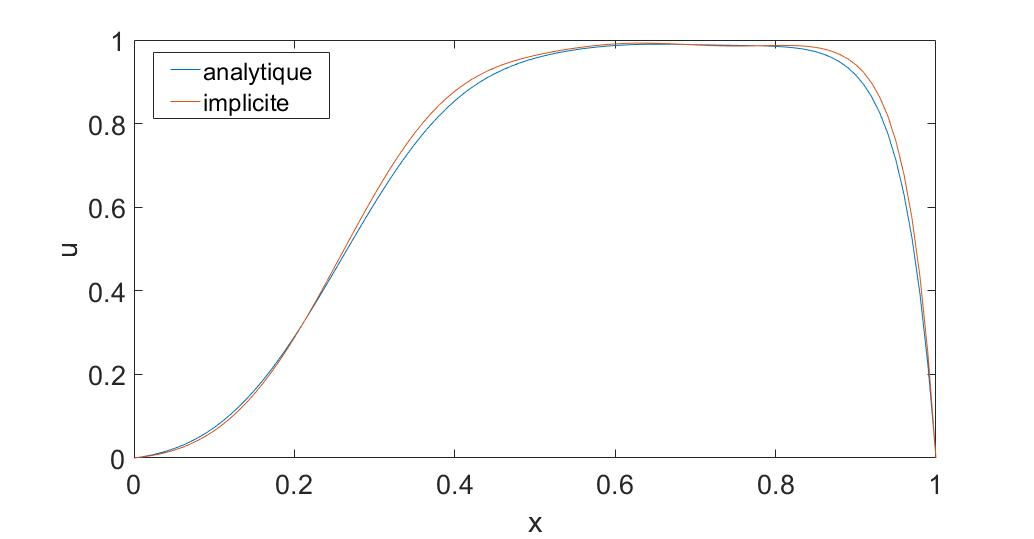
\includegraphics[scale=0.4]{images/analy_vs_impl_t_end_0dot01.jpg}
  \caption{Comparaison entre les solutions analytique et numérique implicite pour
  les paramètres $a=25$, $b=1$, $D=1$, $h=0.01$ et $k=0.00001$, au temps $t=0.01$.}
\end{figure}

\begin{figure}[H]
  \center
  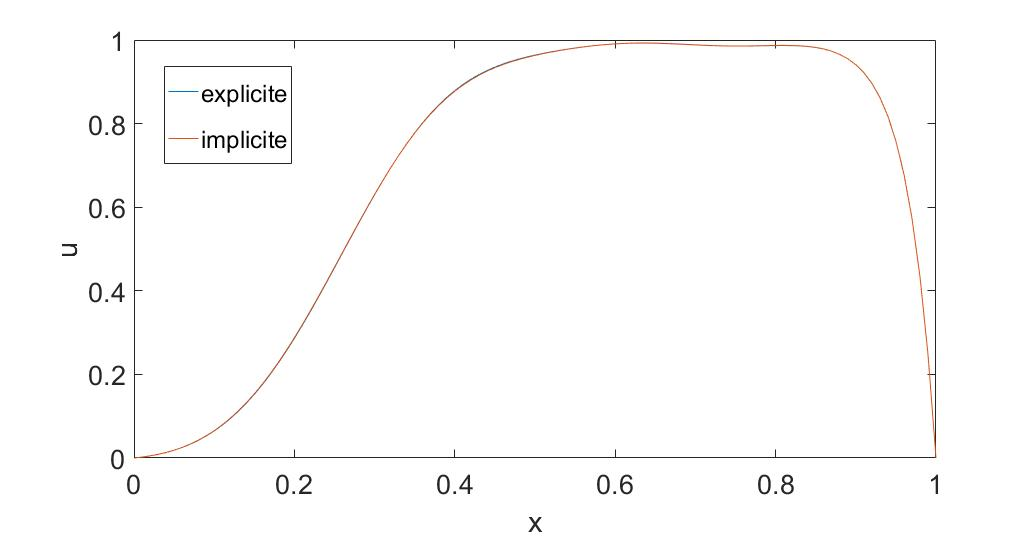
\includegraphics[scale=0.4]{images/expl_vs_impl_t_end_0dot01.jpg}
  \caption{Comparaison entre les solutions numériques implicite et explicite pour
  les paramètres $a=25$, $b=1$, $D=1$, $h=0.01$ et $k=0.00001$, au temps $t=0.01$.}
  \label{eq:expl_vs_impl_t0dot01}
\end{figure}

On peut constater sur les Figures~\ref{eq:expl_vs_impl_t0dot003} et~\ref{eq:expl_vs_impl_t0dot01}
que les solutions numériques implicite et explicite sont quasi identiques pour
les paramètres, conditions aux bords et conditions initiales choisis.

On peut également constanter que dans certains cas, lorsque notre condition pessimiste
de stabilité pour la méthode explicite est violée, le comportement est
effectivement instable (voir Figure~\ref{eq:expl_instable}). En effet,
pour $a=1$, $b=-10$, $D=10$, $h=0.01$ et $k=0.00001$, on a $\lambda_a = 1000$,
$\lambda_b = -0.0001$ et $\lambda_d = 1$. Dès lors,
$|1-\lambda_b| = 1.0001 < |1-\lambda_b + 2 (\lambda_a-2\lambda_d)| = 1997$
et la condition pessimiste de stabilité est donnée par l'Equation~\ref{eq:expl_stabilite_cond_2}.
Ell est en effet non respectée:

\begin{equation}
\left ( 1+2(\lambda_a-2\lambda_d) - \lambda_b \right )^2 + \lambda_a^2 = 4988009 > 1 \;.
\end{equation}

\begin{figure}[H]
  \center
  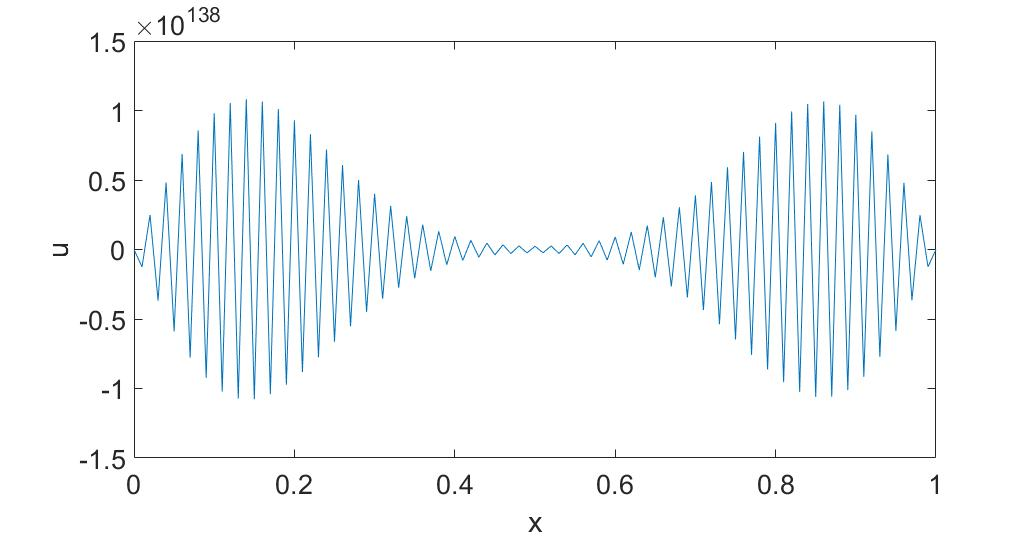
\includegraphics[scale=0.4]{images/expl_instable_a1_b-10_D10_h0dot01_k0dot00001_tend_0dot003.jpg}
  \caption{Instabilité de la méthode numérique explicite pour $a=1$, $b=-10$, $D=10$, $h=0.01$ et $k=0.00001$, au temps $t=0.003$.}
  \label{eq:expl_instable}
\end{figure}

Cependant, on constate que la méthode implicite est elle stable pour ces
paramètres (voir Figure~\ref{eq:impl_stable}).

\begin{figure}[H]
  \center
  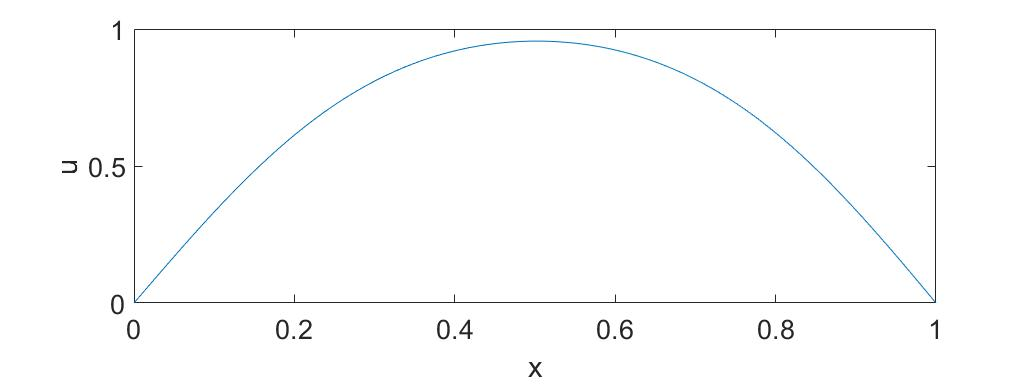
\includegraphics[scale=0.4]{images/impl_stable_a1_b-10_D10_h0dot01_k0dot00001_tend_0dot003.jpg}
  \caption{Stabilité de la méthode numérique implicite pour $a=1$, $b=-10$, $D=10$, $h=0.01$ et $k=0.00001$, au temps $t=0.003$.}
  \label{eq:impl_stable}
\end{figure}

Par contre, confirmant notre réponse à la question 1.4 (voir Section~\ref{sec:implicite}), la méthode implicite
n'est en effet pas toujours stable comme le montre la Figure~\ref{eq:impl_instable}.

\begin{figure}[H]
  \center
  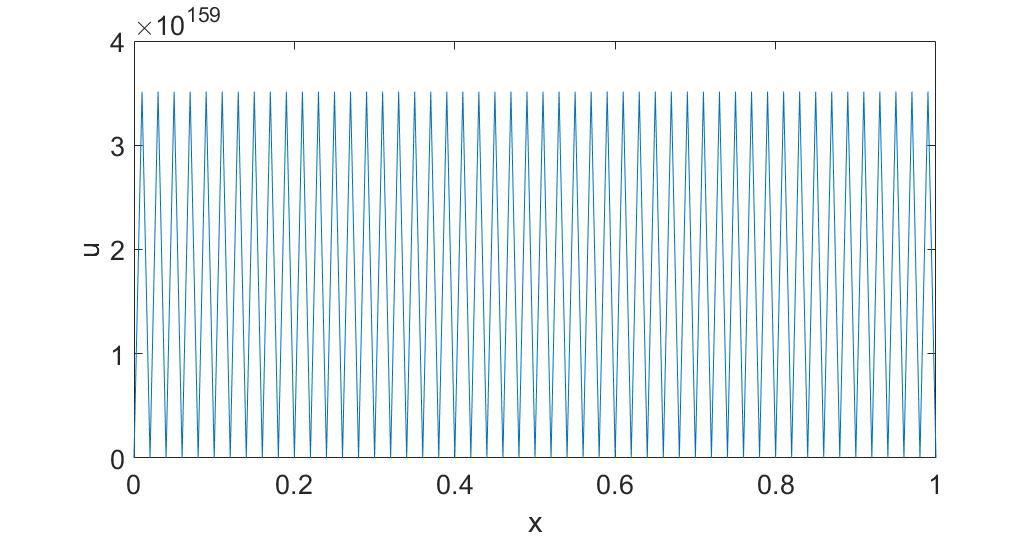
\includegraphics[scale=0.4]{images/impl_instable_a1_b-1divk_D0dot005_h0dot01_k0dot00001.jpg}
  \caption{Instabilité de la méthode numérique implicite pour $\lambda_d = \lambda_a/2$, $\lambda_b = -1$ et $\lambda_a < 1$.}
  \label{eq:impl_instable}
\end{figure}


\section{Montrez, dans ces schéma numériques, quels termes sont responsables de la diffusion numérique. Quel est son ordre de grandeur par rapport à la diffusion explicitement modélisée par le terme D ?}

\subsection*{Schéma explicite}

Afin de déterminer les termes responsables d'une éventuelle diffusion
numérique, calculons l'erreur de troncature $\tau_{i,j}$. Pour rappel
notre schéma numérique explicite a la forme:

\begin{equation}
  U_{\textsl{i},\textsl{j}+1} = U_{\textsl{i}+1, \textsl{j}} (\lambda_d - \lambda_a) + U_{\textsl{i},\textsl{j}} (-2 \lambda_d + \lambda_a - \lambda_b +1) + U_{\textsl{i}-1,\textsl{j}} \lambda_d + \mathcal{O}(k+h) \;.
\end{equation}

Ou encore,

\begin{equation}
  u(x_{\textsl{i}},t_{\textsl{j}}+k) = A u(x_{\textsl{i}}+h, t_{\textsl{j}}) + B u(x_{\textsl{i}}, t_{\textsl{j}}) + C u(x_{\textsl{i}}-h, t_{\textsl{j}}) + k \tau_{i,j}\;.
\end{equation}

Dès lors l'erreur de troncature $\tau_{i,j}$ peut-être exprimée comme:

\begin{equation}
\tau_{i,j} = \frac{1}{k} \left (u(x_{\textsl{i}},t_{\textsl{j}}+k) - A u(x_{\textsl{i}}+h, t_{\textsl{j}}) - B u(x_{\textsl{i}}, t_{\textsl{j}}) - C u(x_{\textsl{i}}-h, t_{\textsl{j}})  \right ) \;.
\label{eq:erreur_troncature}
\end{equation}

On peut développer en séries $u(x_{\textsl{i}},t_{\textsl{j}}+k)$, $u(x_{\textsl{i}}+h, t_{\textsl{j}})$, $u(x_{\textsl{i}}, t_{\textsl{j}})$ et $u(x_{\textsl{i}}-h, t_{\textsl{j}})$,
en gardant uniquement les termes jusqu'à l'ordre $k$ de sorte que on ne considère que
les termes dominant de l'erreur. C'est à dire qu'on calcule $k\tau_{i,j}$ à l'ordre $\mathcal{O}(k)$.

\begin{equation}
  u(x_{\textsl{i}},t_{\textsl{j}}+k) = u(x_{\textsl{i}},t_{\textsl{j}}) + k \frac{\partial u(x_{\textsl{i}},t_{\textsl{j}})}{\partial t} + \mathcal{O}(k^2)
\end{equation}

Par définition de l'équation d'advection-diffusion (Equation~\ref{eq:adv_diff}),
on a:

\begin{equation}
  \frac{\partial u(x_{\textsl{i}},t_{\textsl{j}})}{\partial t} = D \frac{\partial^2 u(x_{\textsl{i}},t_{\textsl{j}})}{\partial x^2} - a \frac{\partial u(x_{\textsl{i}},t_{\textsl{j}})}{\partial x} - b u(x_{\textsl{i}},t_{\textsl{j}}) \;.
  \label{eq:adv_isole_der_par_rap_temps}
\end{equation}

Dès lors,

\begin{equation}
  u(x_{\textsl{i}},t_{\textsl{j}}+k) = u(x_{\textsl{i}},t_{\textsl{j}}) + k \left ( D \frac{\partial^2 u(x_{\textsl{i}},t_{\textsl{j}})}{\partial x^2} - a \frac{\partial u(x_{\textsl{i}},t_{\textsl{j}})}{\partial x} - b u(x_{\textsl{i}},t_{\textsl{j}}) \right ) + \mathcal{O}(k^2)\;.
  \label{eq:taylor_u_t_k}
\end{equation}

Par ailleurs,

\begin{equation}
  u(x_{\textsl{i}} \pm h,t_{\textsl{j}}) = u(x_{\textsl{i}},t_{\textsl{j}}) \pm h \frac{\partial u(x_{\textsl{i}},t_{\textsl{j}})}{\partial x} + \frac{h^2}{2} \frac{\partial^2 u(x_{\textsl{i}},t_{\textsl{j}})}{\partial x^2} \pm \frac{h^3}{6} \frac{\partial^3 u(x_{\textsl{i}},t_{\textsl{j}})}{\partial x^3} + \mathcal{O}(h^4)\;.
  \label{eq:taylor_u_x_h}
\end{equation}

En injectant les Equations~\ref{eq:taylor_u_t_k} et~\ref{eq:taylor_u_x_h} dans
l'expression de l'erreur de troncature (Equation~\ref{eq:erreur_troncature}) on
obtient:

\begin{multline}
  \tau_{i,j} = \frac{1}{k} \left (u(x_{\textsl{i}},t_{\textsl{j}}) (1-bk-A-B-C) + \frac{\partial u(x_{\textsl{i}},t_{\textsl{j}})}{\partial x} (-ak -Ah + Ch) \right.\\
   \left. + \frac{\partial^2 u(x_{\textsl{i}},t_{\textsl{j}})}{\partial x^2} \left (Dk - \frac{A h^2}{2} - \frac{C h^2}{2} \right ) + \frac{\partial^3 u(x_{\textsl{i}},t_{\textsl{j}})}{\partial x^3} \left (-\frac{Ah^3}{6} + \frac{C h^3}{6} \right )  \right ) + \mathcal{O}(k^2+h^4)\;.
   \label{eq:tau_isole}
\end{multline}

Dans notre schéma explicite on a:

\begin{align}
  A = \lambda_d - \lambda_a = \frac{Dk}{h^2} - \frac{ak}{h}\\
  B = -2 \lambda_d + \lambda_a - \lambda_b +1 = -2 \frac{Dk}{h^2} + \frac{ak}{h} - bk +1\\
  C = \lambda_d = \frac{Dk}{h^2}\;.
\end{align}

En injectant ces valeurs de $A,B$ et $C$ dans l'Equation~\ref{eq:tau_isole} on obtient:

\begin{multline}
  \tau_{i,j} = \frac{1}{k} \left ( \frac{\lambda_a h^2}{2} \frac{\partial^2 u(x_{\textsl{i}},t_{\textsl{j}})}{\partial x^2} + \frac{\lambda_a h^3}{6} \frac{\partial^3 u(x_{\textsl{i}},t_{\textsl{j}})}{\partial x^3} \right)\\
  = \frac{a h}{2} \left ( \frac{\partial^2 u(x_{\textsl{i}},t_{\textsl{j}})}{\partial x^2} + \frac{h}{3} \frac{\partial^3 u(x_{\textsl{i}},t_{\textsl{j}})}{\partial x^3} \right ) \;.
\end{multline}

On voit donc qu'on a bien un effet de diffusion numérique lié au terme

\begin{equation}
  \frac{a h}{2} \frac{\partial^2 u(x_{\textsl{i}},t_{\textsl{j}})}{\partial x^2}
  \label{eq:terme_diffusion_numerique}
\end{equation}

de l'erreur de troncature. On voit en effet que ce terme contient une dérivée
seconde de $u$ par rapport à la variable spatiale $x$, tout comme le terme
de diffusion explicitement modélisée

\begin{equation}
  D \frac{\partial^2 u(x_{\textsl{i}},t_{\textsl{j}})}{\partial x^2}\;.
\end{equation}

La constante $a$ ainsi que le pas d'espace $h$ vont influencer l'effet
de diffusion numérique. Si on regarde l'ordre de grandeur relatif entre
la diffusion numérique et la diffusion modélisée explicitement on a:

\begin{equation}
  \frac{\lambda_a h^2 /2}{\lambda_d} = \frac{a h^3}{2D}\;.
\end{equation}

Lorsque $a<0$, le terme de diffusion numérique (Equation~\ref{eq:terme_diffusion_numerique})
a pour d'effet de diminuer l'amplitude de la solution par
rapport à la solution analytique (voir Figure~\ref{eq:expl_diff_num_a_neg}).

\begin{figure}[H]
  \center
  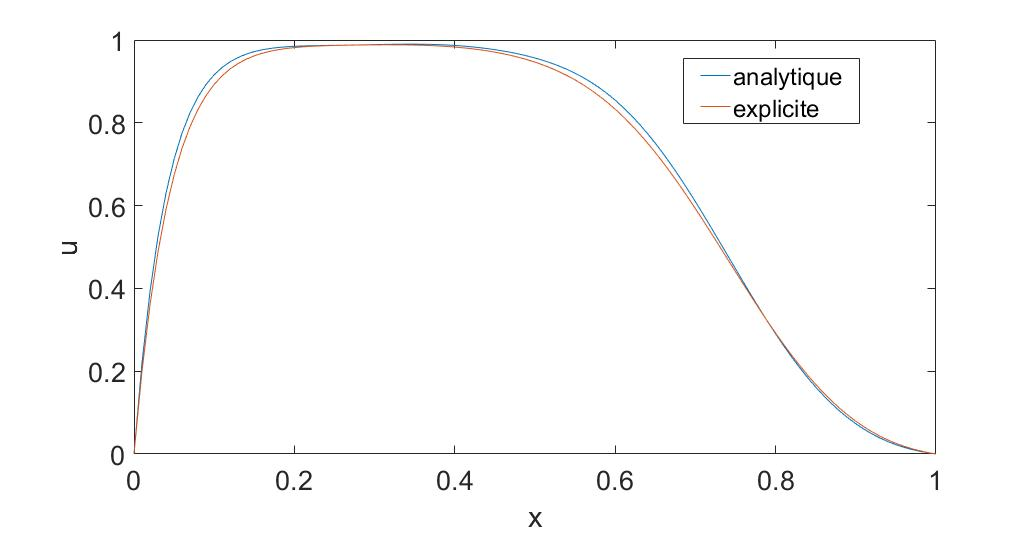
\includegraphics[scale=0.4]{images/expl_diffusion_num_a_neg.jpg}
  \caption{Diffusion numérique du schéma explcite avec $a=-25$, $b=1$, $D=1$,
  $l=1$, $h=0.01$, $k = 0.0000001$ à t=$0.01$.}
  \label{eq:expl_diff_num_a_neg}
\end{figure}

Lorsque $a>0$, le terme de diffusion numérique (Equation~\ref{eq:terme_diffusion_numerique})
a pour d'effet d'augmenter l'amplitude de la solution par
rapport à la solution analytique (voir Figure~\ref{eq:expl_diff_num_higher_h}).

\begin{figure}[H]
  \center
  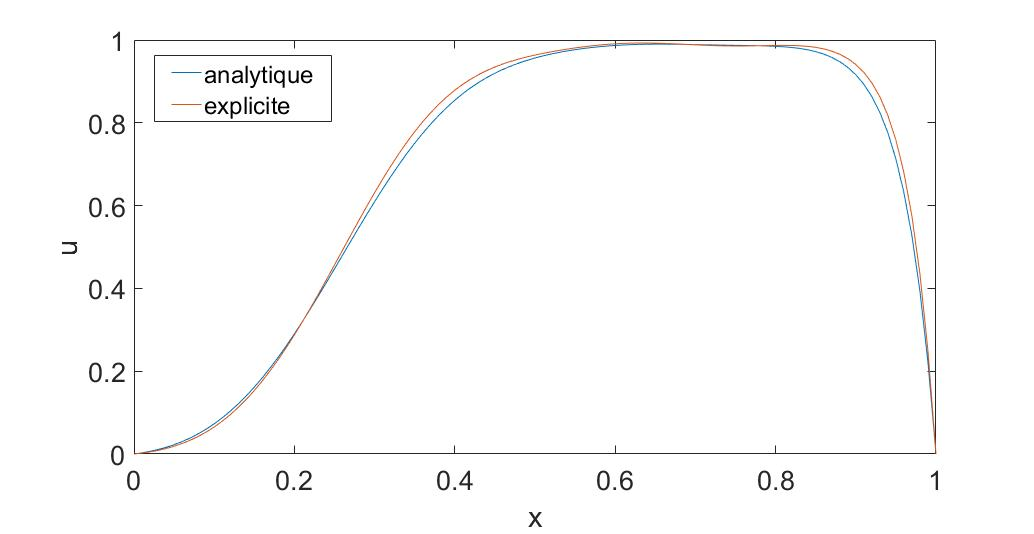
\includegraphics[scale=0.4]{images/expl_diffusion_num_higher_h.jpg}
  \caption{Diffusion numérique du schéma explcite avec $a=25$, $b=1$, $D=1$,
  $l=1$, $h=0.01$, $k = 0.0000001$ à t=$0.01$.}
  \label{eq:expl_diff_num_higher_h}
\end{figure}

On voit que cet effet est moins important lorsque on diminue le pas d'espace $h$,
comme cela est prédit par l'Equation~\ref{eq:terme_diffusion_numerique} (voir Figure~\ref{eq:expl_diff_num}).

\begin{figure}[H]
  \center
  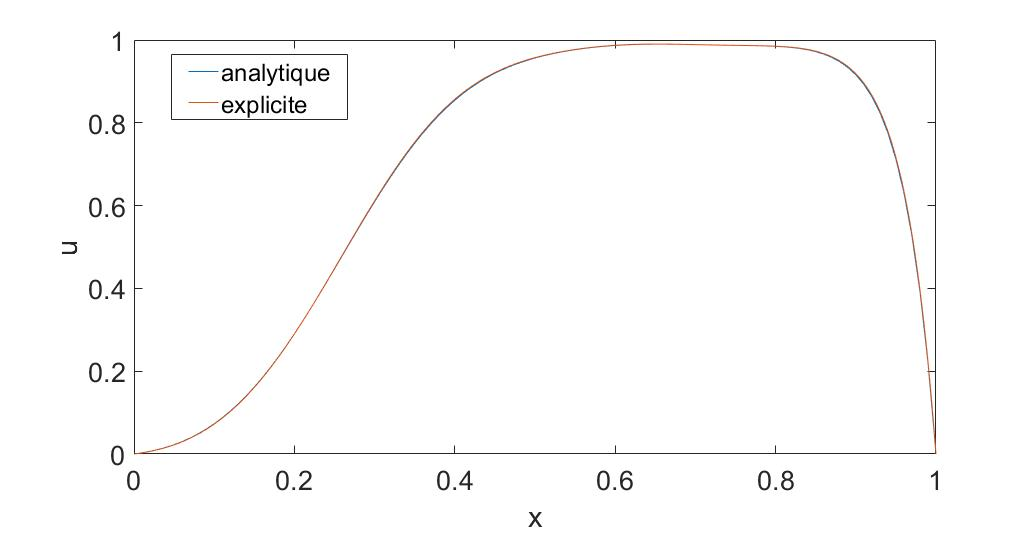
\includegraphics[scale=0.4]{images/expl_diffusion_num.jpg}
  \caption{La diffusion numérique du schéma explcite est moins marquée quand on augmente le pas d'espace. $a=25$, $b=1$, $D=1$,
  $l=1$, $h=0.001$, $k = 0.0000001$ à t=$0.01$.}
  \label{eq:expl_diff_num}
\end{figure}

L'autre terme de l'erreur de troncature à l'ordre considéré, qui fait intervenir une dérivée troisième
en $x$, introduira lui un effet de dispersion.

\subsection*{Schéma implicite}

Une démarche similaire peut-être effectuée pour le schéma implicite. Celui-ci
a la forme:

\begin{equation}
  U_{\textsl{i},\textsl{j}} = A U_{\textsl{i+1},\textsl{j+1}} +  B U_{\textsl{i},\textsl{j+1}} + C U_{\textsl{i-1},\textsl{j+1}}\;.
\end{equation}

Ou encore,

\begin{equation}
u(x_{\textsl{i}}, t_{\textsl{j}}) = A u(x_{\textsl{i}}+h, t_{\textsl{j}}+k) + B u(x_{\textsl{i}}, t_{\textsl{j}}+k) + C u(x_{\textsl{i}}-h, t_{\textsl{j}}+k) + k \tau_{i,j}\;.
\end{equation}

Dès lors en isolant $\tau_{i,j}$ on a:

\begin{equation}
\tau_{i,j} = \frac{1}{k} \left ( u(x_{\textsl{i}}, t_{\textsl{j}}) - A u(x_{\textsl{i}}+h, t_{\textsl{j}}+k) - B u(x_{\textsl{i}}, t_{\textsl{j}}+k) - C u(x_{\textsl{i}}-h, t_{\textsl{j}}+k) \right ) \;.
\end{equation}

On peut remplacer $u(x_{\textsl{i}}, t_{\textsl{j}})$ par un développement en série:

\begin{equation}
  u(x_{\textsl{i}}, t_{\textsl{j}}) = u(x_{\textsl{i}}, t_{\textsl{j}}+k)
  -k \frac{\partial u(x_{\textsl{i}}, t_{\textsl{j}}+k)}{\partial t} + ...\;.
\end{equation}

En remplaçant la dérivée par rapport au temps par l'Equation~\ref{eq:adv_isole_der_par_rap_temps} on a:

\begin{equation}
  u(x_{\textsl{i}}, t_{\textsl{j}}) = u(x_{\textsl{i}}, t_{\textsl{j}}+k)
  -k \left ( D \frac{\partial^2 u(x_{\textsl{i}}, t_{\textsl{j}}+k)}{\partial x^2} - a \frac{\partial u(x_{\textsl{i}}, t_{\textsl{j}}+k)}{\partial x} -b u(x_{\textsl{i}}, t_{\textsl{j}}+k) \right ) + ...\;.
\end{equation}

De plus, les termes $u(x_{\textsl{i}}+h, t_{\textsl{j}}+k)$ et $u(x_{\textsl{i}}-h, t_{\textsl{j}}+k)$
sont remplacés par un développement de Taylor similaire à l'Equation~\ref{eq:taylor_u_x_h}.
On obtient alors:

\begin{multline}
  \tau_{i,j} = \frac{1}{k} \left (u(x_{\textsl{i}}, t_{\textsl{j}}+k) (1+kb-A-B-C) + \frac{\partial u(x_{\textsl{i}}, t_{\textsl{j}}+k)}{\partial x}  ( ka -Ah +Ch ) \right. \\
  \left. + \frac{\partial^2 u(x_{\textsl{i}}, t_{\textsl{j}}+k)}{\partial x^2} \left (-kD - \frac{A h^2}{2} - \frac{Ch^2}{2} \right ) + \frac{\partial^3 u(x_{\textsl{i}}, t_{\textsl{j}}+k)}{\partial x^3}  \left (-\frac{A h^3}{6} + \frac{Ch^3}{6} \right ) \right )\;.
\end{multline}

Pour notre schéma implicite on a $A = \lambda_a - \lambda_d$, $B = 1+2\lambda_d + \lambda_b-\lambda_a$ et $C=-\lambda_d$.
En injectant ces valeurs, les termes en $u$ et en derivée première de $u$ par rapport
à $x$ se simplifient. Le terme de troncature devient donc:

\begin{equation}
  \tau_{i,j} = -\frac{h^2 \lambda_a}{2k} \left (\frac{\partial^2 u(x_{\textsl{i}}, t_{\textsl{j}}+k)}{\partial x^2} + \frac{h}{3} \frac{\partial^3 u(x_{\textsl{i}}, t_{\textsl{j}}+k)}{\partial x^3}  \right )\;.
\end{equation}

On obtient donc un terme de diffusion numérique identique en valeur absolue,
mais de signe opposé, à celui obtenu pour la méthode explicite. Son ordre
de grandeur en valeur absolue par rapport au terme de diffusion explicitement
modélisée est donc le même que pour la méthode explicite. %La différence de signe
%va induire un effet inverse de diffusion numérique par rapport à la méthode
%explicite. Lorsque les paramètres sont tels que la diffusion numérique de la
%méthode explicite induit une plus grande amplitude de la solution numérique par
%rapport à la solution analytique, la diffusion numérique de la méthode implicite
%aura tendance à diminuer l'amplitude par rapport à la solution analytique.


\section{Comparez vitesse de groupe numérique avec celle du système original. Le schéma est-il dispersif?}

\subsection*{vitesse de groupe analytique}

A partir de la définition de la vitesse de groupe :

\begin{equation}
 v_{g} \equiv \frac{d\omega_{r}}{dk}
\end{equation}

où $\omega_{r}$ est la partie réelle de la relation de dispersion \eqref{eq:dispersion}, on obtient :

\begin{equation}
 v_{g} = a\;.
\end{equation}

\subsection*{vitesse de groupe numérique}

On part d'une expression discrète d'une onde plane :

\begin{equation}
  U_{\textsl{i},\textsl{j}} = e^{i\left(\bar{k}x_{\textsl{i}}-\omega t_{\textsl{j}}\right)}
\end{equation}

où l'on distinguera le nombre d'onde $\bar{k}$ du pas de temps $k$. On l'injecte dans l'équation aux différences explicite \eqref{eq:schema_num_sans_erreur} de notre équation différentielle de départ. On obtient :

\begin{equation}
  e^{i\left(\bar{k}x_{\textsl{i}}-\omega t_{\textsl{j+1}}\right)} = e^{i\left(\bar{k}x_{\textsl{i}-1}-\omega t_{\textsl{j}}\right)} \lambda_d + e^{i\left(\bar{k}x_{\textsl{i}}-\omega t_{\textsl{j}}\right)} (-2 \lambda_d + \lambda_a - \lambda_b +1) + e^{i\left(\bar{k}x_{\textsl{i}+1}-\omega t_{\textsl{j}}\right)} (\lambda_d - \lambda_a)\;.
\end{equation}

En tenant compte du pas d'espace $x_{\textsl{i+1}}- x_{\textsl{i}}= h$ et du pas de temps $t_{\textsl{j+1}}- t_{\textsl{j}}= k$, après calcul on a :

\begin{equation}
  e^{-i\omega k} = e^{-i\bar{k}h} \lambda_d + (-2 \lambda_d + \lambda_a - \lambda_b +1) + e^{i\bar{k}h} (\lambda_d - \lambda_a) \;.
  \end{equation}

 Nous allons faire une approximation par le théorème de Taylor à l'ordre $\mathcal{O}(h+k)$, en tenant compte que $\bar{k}$ et les $\lambda$ sont fixés, nous obtenons :

 \begin{eqnarray*}
  1-i\omega k &=& (1-i\bar{k}h) \lambda_d + (-2 \lambda_d + \lambda_a - \lambda_b +1) + (1+i\bar{k}h) (\lambda_d - \lambda_a)\\
  &=& \lambda_d -i\bar{k}h \lambda_d - 2 \lambda_d + \lambda_a - \lambda_b + 1 + \lambda_d + i\bar{k}h \lambda_d - \lambda_a - i\bar{k}h \lambda_a \;.
  \end{eqnarray*}

  Après simplification et en remplaçant $\lambda_a$ par sa valeur $\lambda_a = \frac{ak}{h}$, on obtient :

  \begin{eqnarray}
  \omega  &=& \frac{\bar{k}h}{k}\lambda_a\\
	&=& a\bar{k}\;.
  \end{eqnarray}

   Nous calculons la vitesse de groupe numérique par différence avant, on obtient :

  \begin{eqnarray}
     v_{gn} &=& \frac{d\omega}{d\bar{k}}\\
     &=& a \frac{d\bar{k}}{d\bar{k}}\\
     &=& a \;.
  \end{eqnarray}

  Cette approximation à l'ordre $\mathcal{O}(h+k)$, nous permet de retrouver la vitesse de groupe analytique.

\subsection*{Schéma non dispersif au premier ordre}

La vitesse de groupe numérique n'est pas fonction de $\bar{k}$,
elle est égale à une constante $a$ dans notre approximation.
Notre schéma n'est donc pas dispersif au premier ordre.
Ce qui est cohérent avec notre système originel qui est non dispersif $v_{g} = a $.


\section{Le terme de diffusion D peut-il être responsable d'un comportement instable? Expliquer.}

Oui car le terme $\lambda_D  = Dk /h^2$ apparait dans les conditions de A-stabilité
des schémas numériques explicites et implicites.

Pour le schéma explicite,
en regardant l'Equation~\ref{eq:kappa_squared}, on voit que plus on augmente
la valeur de $D$ (et donc de $\lambda_D$) plus on tend avec certitude vers
une situation où l'inégalité (et donc la condition de stabilité) n'est pas
satisfaite. En effet, alors que pour une certaine combinaison des paramètres
, dont $D=5$, la méthode explicite présente un comportement stable (voir
Figure~\ref{eq:stable_Q7}), elle ne l'est pas si on augmente la valeur de $D$ à $6$
(voir Figure~\ref{eq:instable_Q7}).

\begin{figure}[H]
  \center
  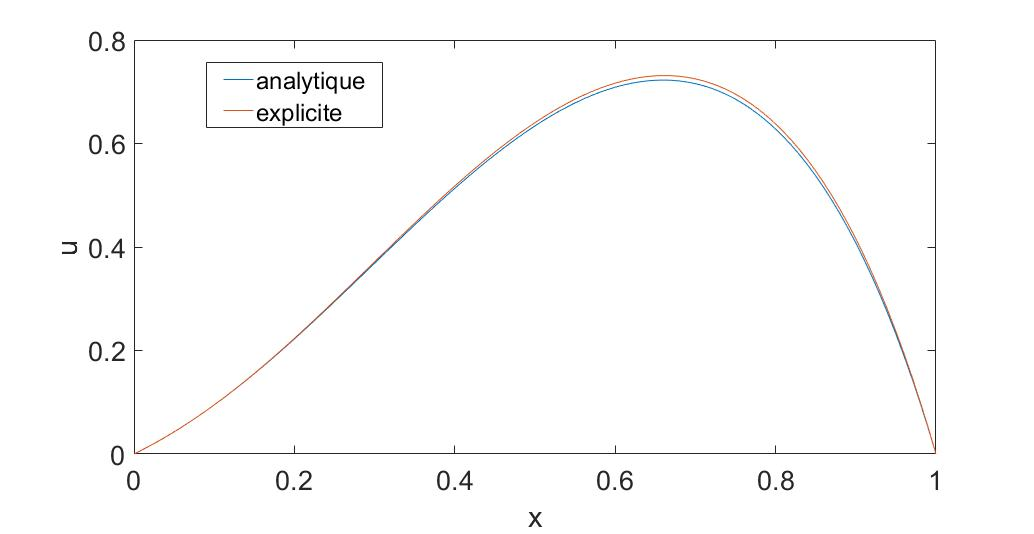
\includegraphics[scale=0.4]{images/q7D5stable.jpg}
  \caption{Méthode explicite stable pour $a=25$, $b=5$, $D=5$,
  $l=1$, $h=0.01$, $k = 0.00001$ à t=$0.01$.}
  \label{eq:stable_Q7}
\end{figure}

\begin{figure}[H]
  \center
  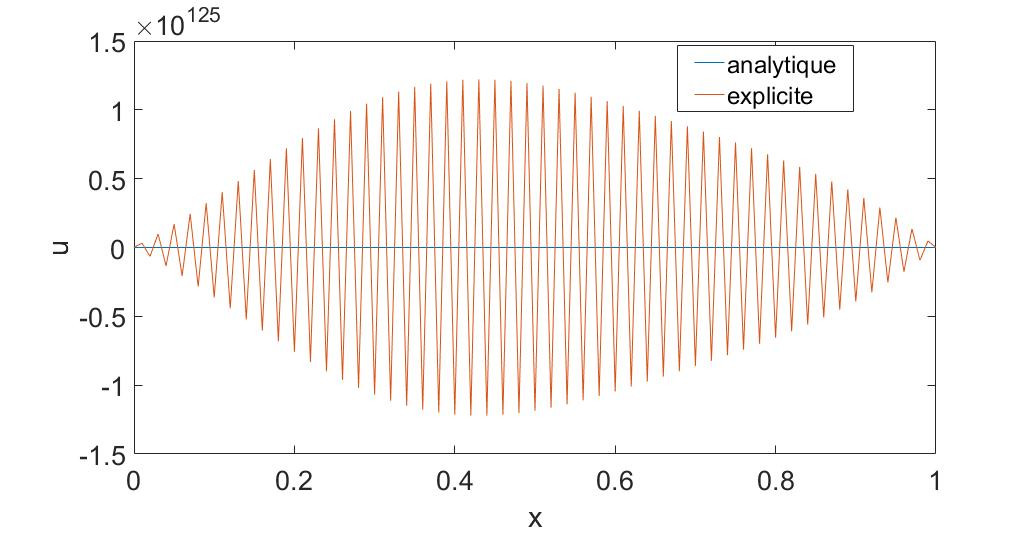
\includegraphics[scale=0.4]{images/q7D6instable.jpg}
  \caption{Méthode explicite instable pour $a=25$, $b=5$, $D=6$,
  $l=1$, $h=0.01$, $k = 0.00001$ à t=$0.01$.}
  \label{eq:instable_Q7}
\end{figure}

Pour le schéma implicite, varier $D$ et donc le terme $\lambda_d$ peut également
engendrer non-satisfaction de la condition de stabilité. Cependant il y a,
contraitement au cas du schéma explicite, des combinaisons de paramètres pour
lesquelles le schéma sera stable pour toutes les valeurs de $D$ possibles.

\section{Fournissez un schéma de Lax-Wendroff à trois points $\left(\textsl{i}-1,\textsl{i},\textsl{i}+1\right)$ dans l'espace. Quel est l'ordre de ce schéma? Est-il monotone? Discutez les avantages et les inconvénients au schéma que vous avez donné au point 1 ci-dessus.}


Ce schéma de Lax-Wendroff peut-être obtenu en exigeant que l'erreur de troncature
$k \tau_{i,j}$ de l'Equation~\ref{eq:tau_isole} tende vers 0 lorsque $h \to 0$.
L'Equation~\ref{eq:tau_isole} de l'erreur de troncature du schéma explicite
peut se réécrire comme:

\begin{multline}
  k\tau_{i,j} = u(x_{\textsl{i}},t_{\textsl{j}}) (1-\lambda_b-A-B-C) + \frac{\partial u(x_{\textsl{i}},t_{\textsl{j}})}{\partial x} h (-\lambda_a -A + C) \\
   + \frac{\partial^2 u(x_{\textsl{i}},t_{\textsl{j}})}{\partial x^2} \frac{h^2}{2} \left (2 \lambda_d - A - C \right ) + \frac{\partial^3 u(x_{\textsl{i}},t_{\textsl{j}})}{\partial x^3} \frac{h^3}{6} \left (C-A \right )  + \mathcal{O}(k^2+h^4)\;.
   \label{eq:tau_isole2}
\end{multline}

Pour que $k \tau_{i,j} \to 0$ quand $h \to 0$ on doit avoir:

\begin{align}
  1-\lambda_b - A -B -C = 0\\
  -\lambda_a +C - A =0\\
  2 \lambda_d -A -C = 0\;.
\end{align}

En résolvant ce système linéaire on obtient:

\begin{align}
  A = -\frac{\lambda_a}{2} + \lambda_d\\
  B = 1-\lambda_b - 2\lambda_d\\
  C = \frac{\lambda_a}{2} + \lambda_d\;.
\end{align}

Le schéma numérique est donc:

\begin{equation}
U_{\textsl{i},\textsl{j+1}} = \left ( -\frac{\lambda_a}{2} + \lambda_d \right ) U_{\textsl{i+1},\textsl{j}} + B (1-\lambda_b - 2\lambda_d) U_{\textsl{i},\textsl{j}} + \left (\frac{\lambda_a}{2} + \lambda_d \right ) U_{\textsl{i-1},\textsl{j}} \;.
\end{equation}


%\section*{Conclusion}

\part{Prédictibilité}
\setcounter{section}{0}

\section*{Introduction}


\section{todo}


\section*{Conclusion}




\end{document}
